\documentclass[twocolumn, 9pt]{article}
\usepackage[utf8]{inputenc}
\usepackage[T1]{fontenc}
\usepackage{amsmath, amssymb}
\usepackage{graphicx}
\usepackage{booktabs}
\usepackage{algorithm}
\usepackage[noend]{algpseudocode}
\usepackage{listings}
\usepackage{cite}
\usepackage{hyperref}
\usepackage{geometry}
\usepackage{lmodern} % You can change this to a font of your choice
\usepackage{abstract}



% Define the page margins
\geometry{left=20mm, right=20mm, top=25mm, bottom=25mm}

% Define some custom math commands
\newcommand{\vect}[1]{\boldsymbol{#1}} % Vector
\newcommand{\matr}[1]{\mathbf{#1}} % Matrix
\newcommand{\deriv}[2]{\frac{d #1}{d #2}} % Derivative
\newcommand{\pderiv}[2]{\frac{\partial #1}{\partial #2}} % Partial Derivative
\newcommand{\integral}[4]{\int_{#1}^{#2} #3 \, d#4} % Integral

% Pseudocode settings
\algnewcommand\algorithmicinput{\textbf{Input:}}
\algnewcommand\Input{\item[\algorithmicinput]}
\algnewcommand\algorithmicoutput{\textbf{Output:}}
\algnewcommand\Output{\item[\algorithmicoutput]}

% Code listing settings
\lstset{
  basicstyle=\ttfamily,
  columns=fullflexible,
  frame=single,
  breaklines=true,
  postbreak=\mbox{\textcolor{red}{$\hookrightarrow$}\space},
}

\title{Variational Autoencoders}
\author{Sergio Alberto De León Martínez \\ CIMAT}
% \date{\today}


\begin{document}

\fontfamily{cmss}\selectfont


\twocolumn[
  \begin{@twocolumnfalse}
  \maketitle
    \begin{abstract}
    \noindent
   This work explores Variational Autoencoders (VAEs) from a probabilistic perspective and demonstrates their application on the MNIST dataset. The theoretical foundations of VAEs are introduced, including variational inference and training, and experiments are presented to evaluate the quality of reconstruction, visualization, interpolation, and robustness. Additionally, conditional generation and anomaly detection are examined. The study highlights the effectiveness of VAEs in various applications.
    \end{abstract}
    \vspace{1cm} % You can adjust this vertical space or remove it
  \end{@twocolumnfalse}
]

\section{Introduction}
A generative model is one that can simulate a random variable from a learned distribution, examples in (Kingma and Welling 2014\cite{kingma2013auto}). In 2014, the use of Variational Autoencoders (VAE) and Generative Adversarial Networks (GANs) achieved the first practical deep neural networks capable of learning generative models of complex data, such as images \cite{wikipedia_ia_generativa}. Since then, VAEs have been used in a variety of applications ranging from popular cases such as Open-AI's Dall-E model \cite{finetwork_dalle}, to applications in physics for classifying phase transitions in the Ising model \cite{wetzel2017unsupervised}, and even in medicine for inferring the age of a group of patients with magnetic resonance imaging \cite{zhao2019variational}. In this work, we will introduce the Variational Autoencoder model from a probabilistic perspective and then show and explain various experiments with the MNIST dataset.

\section{Variational Inference and Neural Networks}

Consider a dataset $ { x_{i} }$, whose dimensionality is typically very large, making its practical handling very costly. We would like to encode our dataset in such a way that information loss is minimized. Let's denote $ { z_i } $ as the encoded variables, which are often referred to as latent variables. We will assume a probabilistic model for the variables $ x_i, z_i $. The process we would like to follow to obtain samples is as follows, for each data point $ x_i $:

\begin{itemize}
\item Write the latent variable $ z_i \sim p(z)$ \
\item Generate a sample $x_i \sim p(x | z)$
\end{itemize}

Recall that the joint probability of the model can be written as $ p(x, z) = p(x | z)p(z) $, where the distribution of $ x | z$ can be deduced from the data. For example, consider a $28\times28$ pixel black and white image of handwritten numbers. Then, each pixel can be thought of as a random variable that follows a Bernoulli distribution with a parameter to be determined. Similarly, the latent variables are expected to follow a Gaussian distribution with parameters also to be determined. In this context, we would like to infer the values of the latent variables given the dataset as accurately as possible, this is $p(z | x)$ from Bayes' theorem, we have 

$$
p(z | x) = \frac{p(x | z)p(z)}{p(x)}.
$$

The term $p(x)$ is known as the evidence and can be obtained by marginalizing

$$
p(x) = \int p(x | z)p(z) ~ dz
$$

The disadvantage is that this integral is computationally expensive to calculate. Instead, the alternative is to optimize a lower bound.  \\

\subsection{Variational Lower Bound}

Instead of directly calculating $p (z | x)$, it can be approximated with a family of distributions $q_\phi(z | x)$ where the parameterization $\phi$ is given by the weights and biases of a neural network. Continuing with this idea, the distribution of $x | z$ can also be learned from a neural network, that is, consider the family of distributions $p_\theta(x | z)$ where again, $\theta$ represents the weights and biases of a neural network. The way the model will be trained is through the paradigm of maximizing the likelihood $p_\theta(x)$ or alternatively optimizing a lower bound. For this, consider the following calculation. \

We would like to find a lower bound to \(\log p_\theta(x)\):

\begin{align*}
\log p_\theta(x) &= \mathbb{E}_{z\sim q_\phi(z|x)} \log p_\theta(x) \\
&= \mathbb{E}_{z\sim q_\phi(z|x)} \log \frac{p_\theta(x,z)}{p_\theta(z|x)} \\
&= \mathbb{E}_{z\sim q_\phi(z|x)} \log \frac{p_\theta(x,z)}{q_\phi(z|x)} \frac{q_\phi(z|x)}{p_\theta(z | x)} \\
&= \mathbb{E}_{z\sim q_\phi(z|x)} \frac{p_\theta(x,z)}{q_\phi(z|x)} + \mathbb{E}_{z\sim q_\phi(z|x)} \log \frac{q_\phi(z|x)}{p_\theta(z | x)}
\end{align*}

The first term is known as the variational lower bound or the evidence lower bound (ELBO).

$$
\mathcal{L}(\phi, \theta) =  \mathbb{E}_{z\sim q_\phi(z|x)} \frac{p_\theta(x,z)}{q_\phi(z|x)}
$$

The second term is known as the Kullback-Leibler divergence. In general, we have that

\[
D_{KL}(q || p) = \mathbb{E}_{z\sim q} \log \frac{q(z)}{p(z)}
\]

Remarks:
\begin{itemize}
    \item \(D_{KL}(q || p) \neq D_{KL}(p || q)\)
    \item Mide qué tan lejos está \(p\) de \(q\)
    \item \(D_{KL}(q || p) \geq 0\) (y 0 si y sólo si \(p = q\))
\end{itemize}

The last observation follows from Jensen's inequality, which states the following
$$
{\varphi \left(\mathbb {E} \{X\}\right)\leq \mathbb {E} \{\varphi (X)\}.}
$$

For $\varphi$ a convex function. Since the \(K\)-\(L\) divergence is defined positive, then the evidence lower bound (ELBO) is indeed a lower bound of the likelihood:
\[
\log p_\theta(x) \geq \mathbb{E}_{z\sim q_\phi(z|x)} \log \frac{p_\theta(x,z)}{q_\phi(z|x)} = \mathcal{L}_{\theta, \phi}(x)
\]

The ELBO function, \(\mathcal{L}_{\theta,\phi}(x)\), can be broken down as follows:

\begin{align*}
\mathcal{L}_{\theta,\phi}(x) &= \mathbb{E}_{z\sim q_\phi(z|x)} \left[ \log \frac{p_\theta(x,z) }{q_\phi(z|x)} \right] \\
&= \mathbb{E}_{z\sim q_\phi(z|x)} \left[ \log \frac{p_\theta(x|z) p(z)}{q_\phi(z|x)}  \right] \\
&= \mathbb{E}_{z\sim q_\phi(z|x)} \left[ \log p_\theta(x|z) \right] + \mathbb{E}_{z\sim q_\phi(z|x)} \left[ \log \frac{p(z)}{q_\phi(z|x)} \right]
\end{align*}

Consider the first term, if $p_\theta(x|z)\sim\mathcal{N}(x; G_\theta(z), \eta I)$, then

\begin{align*}
\log p_\theta(x|z) &= \log \left[ \frac{1}{\sqrt{(2\pi)^d \eta^d}} \exp\left(-\frac{1}{2}(x - G_\theta(z))^T\eta I(x - G_\theta(z))\right) \right] \\
&= -\frac{1}{2} || x - G_\theta(z) ||^2 + \log \left[ \frac{1}{\sqrt{(2\pi)^d \eta^d}} \right]
\end{align*}

So, the expectation of the logarithm of \(p_\theta(x|z)\) is the mean of the mean squared error of reconstruction under the encoder model. The second term can be thought of as a regularization term, and furthermore, let's see that
\[
\mathbb{E}_{z \sim q_\phi(z|x)} \log \frac{p(z)}{q_\phi(z|x)} = -D_{KL}(q_\phi(z|x) || p(z))
\]

Thus, maximizing ELBO \(\mathcal{L}_{\theta,\phi}\) implies:
\begin{itemize}
    \item Approximately maximizing \(\log p_\theta(x|z)\).
    \item Minimizing the K-L divergence between \(q_\phi(z|x)\) and \(p_\theta(z|x)\) making \(q_\phi\) better.
\end{itemize}

Here is the English translation of your subsection:

\subsection{Training}

Instead of optimizing
\[
\sum_{i=1}^n \log p_\theta(x_i)
\]

Optimize \( \sum_i \mathcal{L}_{\theta,\phi}(x_i)\) with
\[
\mathcal{L}_{\theta,\phi}(x) = \mathbb{E}_{z \sim q_\phi(z|x)} \left[ \log \frac{p_\theta(x,z)}{q_\phi(z|x)} \right]
\]

The parameters of the inference model are shared among the data. Now, calculating $\nabla_{\theta, \phi} \mathcal{L}_{\theta, \phi}(x_i)$ is intractable, but some unbiased estimators can be deduced, for $\theta$ it is simple.

\begin{align*}
\nabla_{\theta} \mathcal{L}_{\theta, \phi}(x) &= \nabla_{\theta} \mathbb{E}_{z \sim q_{\theta}(z|x)} \left[\log p_{\theta}(x, z) - \log q_{\theta}(z|x) \right] \\
&= \mathbb{E}_{z \sim q_{\theta}(z|x)} \nabla_{\theta} \log p_{\theta}(x)   \\
&\approx \nabla_{\theta} \log p_{\theta}(x) \quad \text{with} \quad z \sim q_{\theta}(z|x)
\end{align*}

But for $\phi$ it's not the same, since as it changes, $q_{\phi}(z|x)$ changes as well. However, remember that $q_{\phi}(z|x) \sim \mathcal{N}(z; \mu(x), \sigma(x)\mathbf{I})$, then 

$$
q_{\phi}(z|x) = \mu_(x) + \sigma_(x) \cdot \epsilon \text{ with } \epsilon \sim \mathcal{N}(0, \mathbf{I})
$$

therefore

\begin{align*}
\mathcal{L}_{\theta}(x) &= \mathbb{E}_{z \sim q_{\theta}(z|x)} [\log p_{\theta}(x|z) - \log q_{\phi}(z|x)] \\
&= \mathbb{E}_{\epsilon \sim p(\epsilon)} [\log p_{\theta}(x|z) - \log q_{\phi}(z|x)]
\end{align*}

where in the last expression we have separated the random sources from the differentiable quantities to take it as an unbiased estimator for $\nabla_{\phi} \mathcal{L}_{\theta, \phi}(x)$.

\section{Experiments}

Next, we will show the results of a series of experiments that we conducted with the MNIST dataset, which consists of a series of images of $28\times28$ pixels. The number of hidden layers used and the dimension of the latent space were 256 and 200 respectively. The training was done over 50 epochs.

\subsection{Quality of Reconstruction}

The first thing we did was to pass a set of test images through the VAE and then calculate the average mean squared error between the original and reconstructed images, obtaining the following value:

$$
\textbf{Average MSE:   0.01731714333136813}
$$

Below are some images to make a visual comparison.

\begin{figure}[ht]
\centering
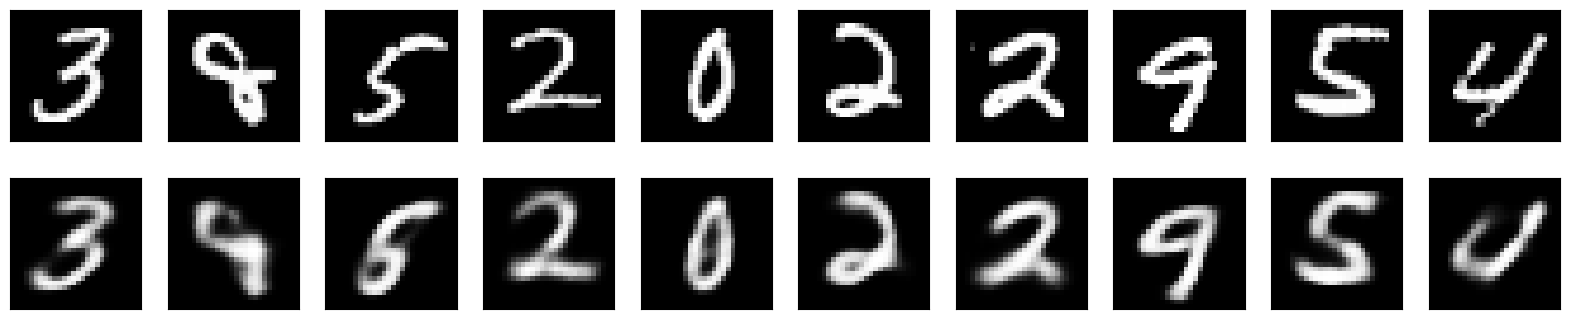
\includegraphics[width=\linewidth]{original_reconstructed.png}
\caption{Up: original image. Below: reconstructed image.}
\label{fig:example}
\end{figure}

\subsection{Visualization}

For this experiment, we set the dimension of the latent space to 2, with the purpose of being able to visualize it and detect patterns that allow us to better understand how the network learns to distinguish between different classes.

\begin{figure}[ht]
\centering
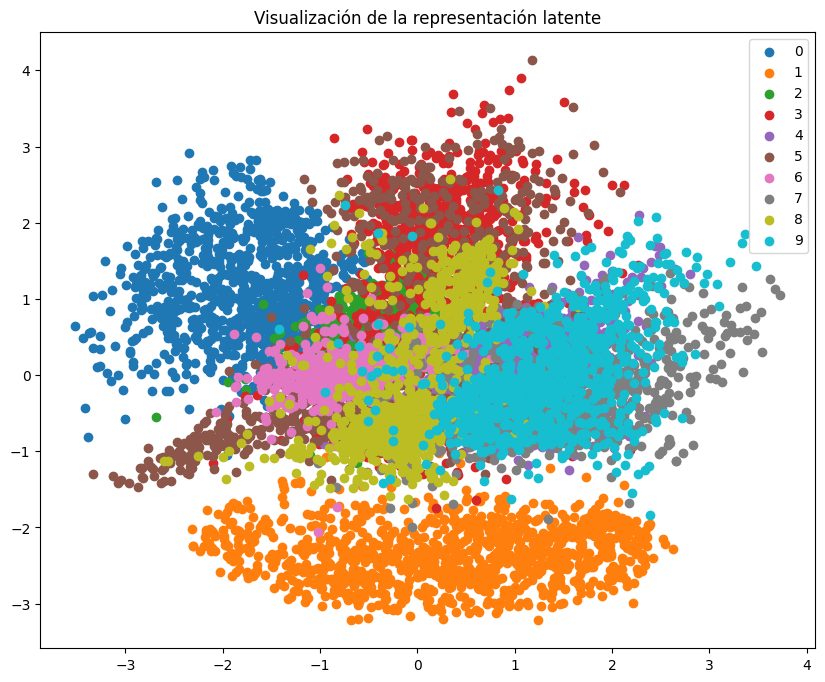
\includegraphics[width=\linewidth]{latent_visualization.png}
\caption{Latent space visualization.}
\label{fig:example2}
\end{figure}

As we can appreciate in Figure \ref{fig:example2}, the representations associated with the same class tend to cluster in the same region. However, we can also see how different clusters overlap, which motivates the following example.

\subsection{Interpolation}

Let's consider two images of different classes, for example, zero and one. Then, we pass these two images through the encoder to obtain their respective representations in the latent space ($\mu$). Next, we interpolate linearly and use the decoder to obtain a series of images that allow us to see how the network transitions smoothly between classes, as shown in the image below.

\begin{figure}[ht]
\centering
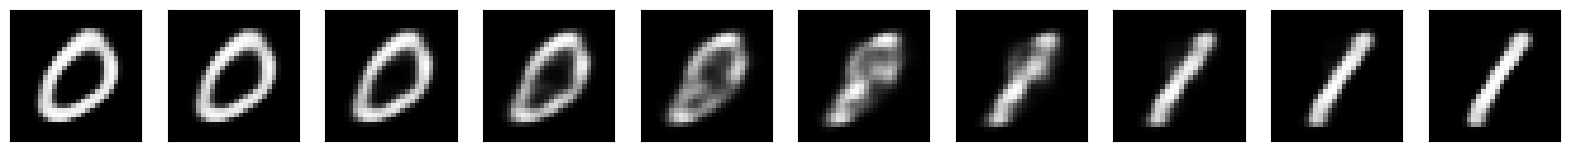
\includegraphics[width=\linewidth]{interpolation.png}
\caption{Interpolation between classes.}
\label{fig:example3}
\end{figure}

\subsection{Robustness}

To test the robustness of the model, we considered a set of test images and applied Gaussian noise to them. Then, we passed them through the VAE for reconstruction and calculated the average mean squared error between the noise-free images and the reconstructed ones, obtaining the following result:

$$
\textbf{Average MSE (with noise): 0.021153034076999172}
$$

Figure \ref{fig:example4} compares the noisy images with their respective reconstructed image.

\begin{figure}[ht]
\centering
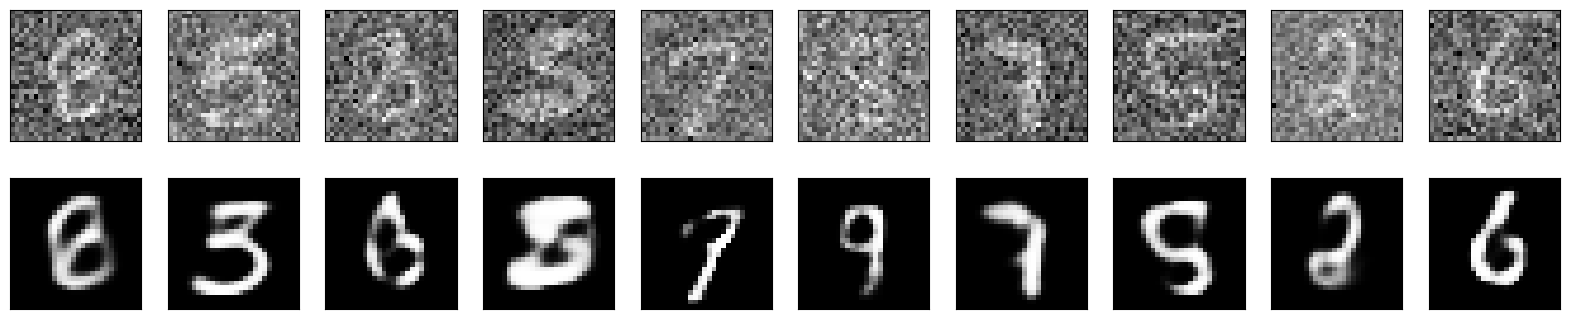
\includegraphics[width=\linewidth]{robustness.png}
\caption{Images with Gaussian noise and their corresponding reconstruction.}
\label{fig:example4}
\end{figure}

As can be seen from the MSE calculation and the visual comparison, the model is relatively efficient even with the noise factor.

\subsection{Anomaly Detection}

To test the model's efficiency in detecting anomalous data, we considered a dataset significantly different from the MNIST dataset, for example, Fashion-MNIST. First, we took a test dataset from MNIST and calculated the empirical distribution of the mean squared error, setting a threshold to determine if a data point is anomalous at $\mu \pm 2\sigma$. This means if the mean squared error of a data point falls outside this interval, it is considered anomalous. To validate this threshold, we took another subset of MNIST and obtained an accuracy of 98.4%. When repeating this procedure with the Fashion-MNIST dataset, we obtained an accuracy of 1.13%, meaning the vast majority of the data fell outside the previously established threshold, indicating that the model correctly classified them as anomalous.

\subsection{Conditional Generation}

Finally, we would like to generate images conditioned on a specific class. For this, we need to slightly modify the model to accept not only the image but also its corresponding label encoded in one-hot. Once this is done, we generate random vectors in the latent space and pass them through the encoder but conditioned to a particular class. The result is as follows.

\begin{figure}[ht]
\centering
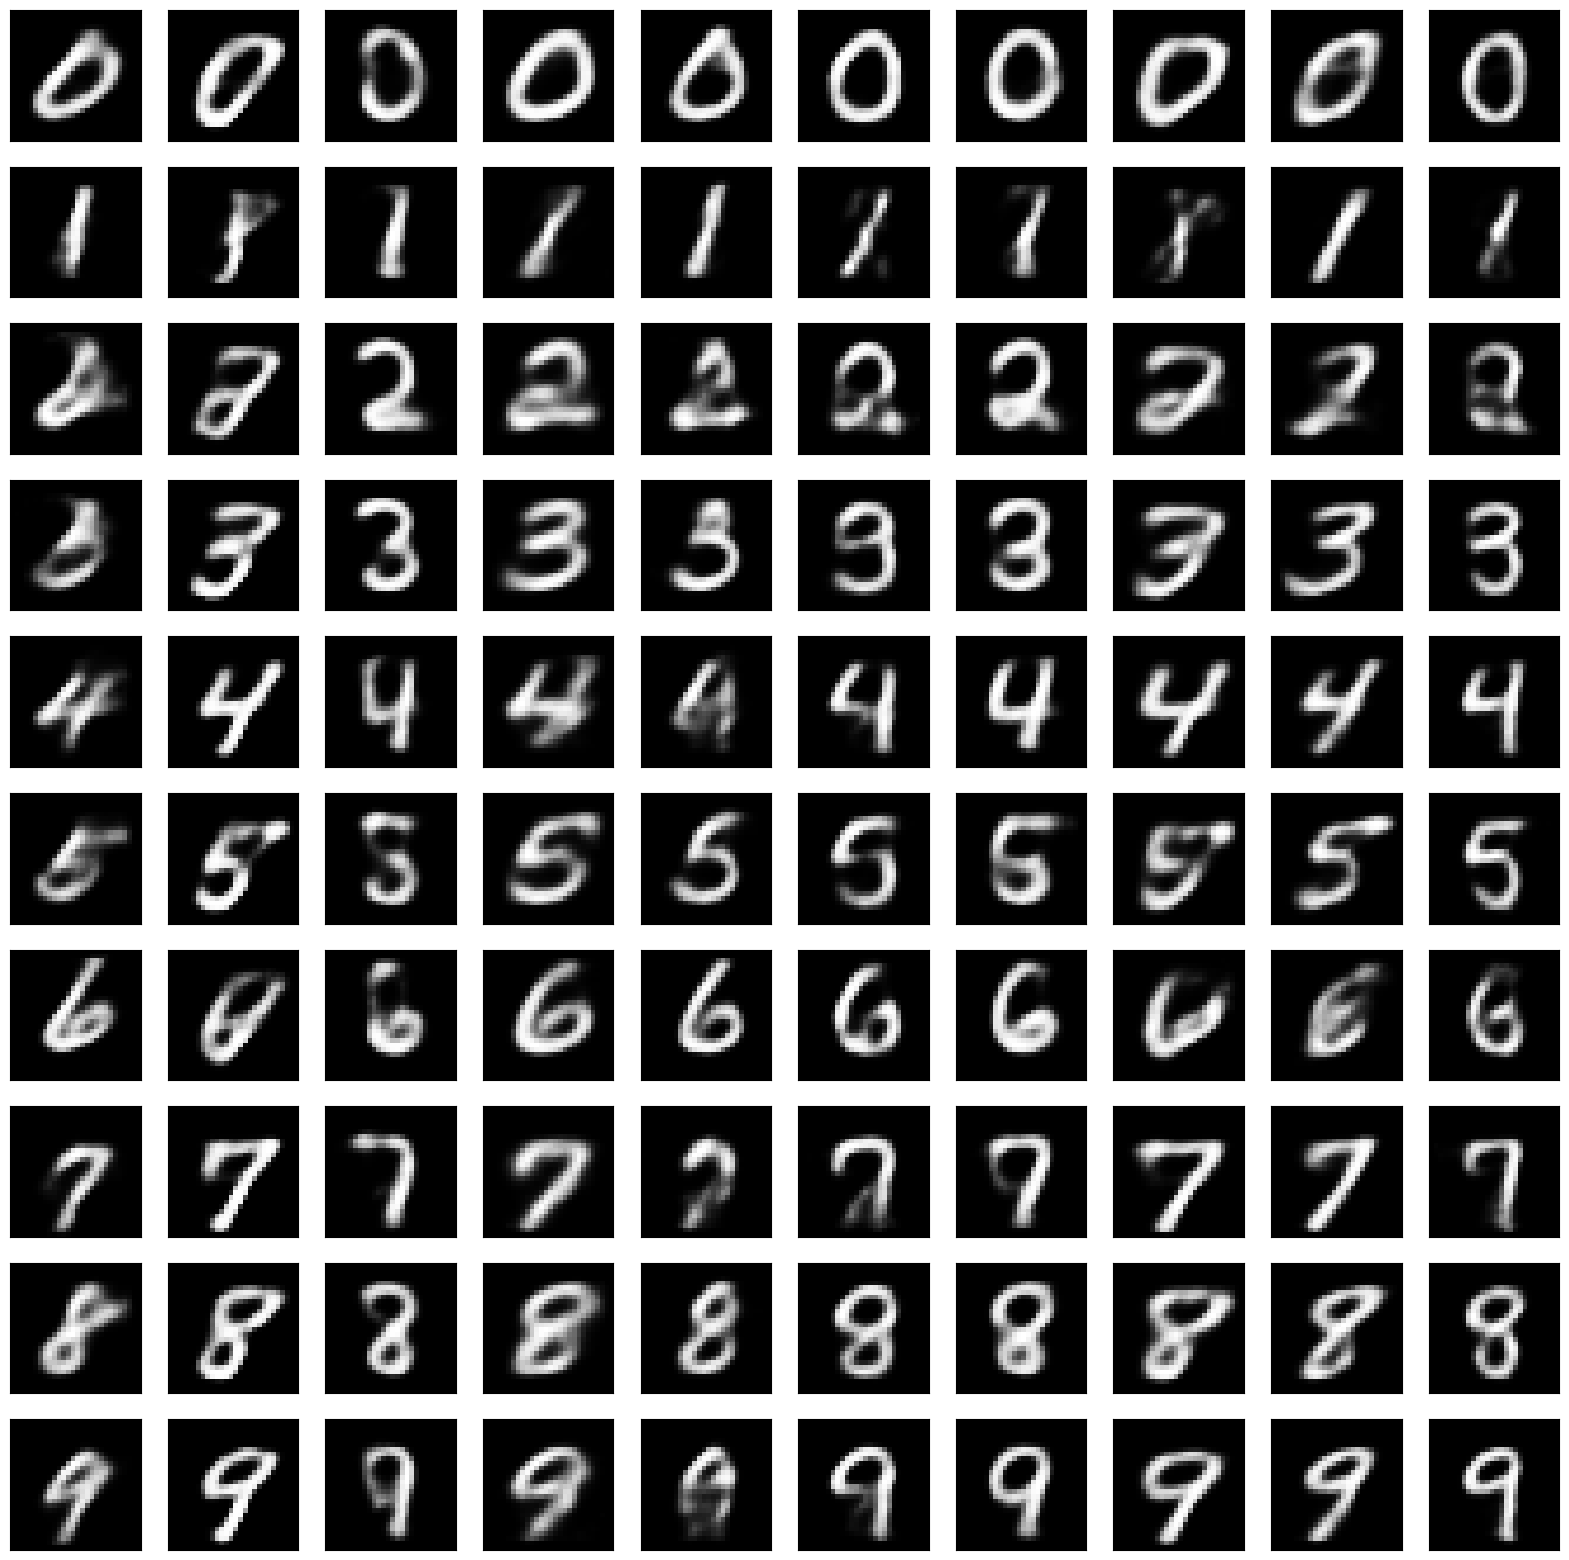
\includegraphics[width=\linewidth]{conditional.png}
\caption{Conditioned images.}
\label{fig:example5}
\end{figure}

In Figure \ref{fig:example5}, different samples conditioned to each of the classes are shown, so we see different examples of 1's, 2's, etc. As a result, we can see an acceptable quality in the images.

\section{Conclusion}

The study on Variational Autoencoders highlights their versatility and efficacy in a wide range of applications. Their ability to generate useful and robust representations is emphasized, demonstrating their potential in areas such as image generation and anomaly detection. The success in these applications suggests that VAEs are powerful and flexible tools for the analysis and interpretation of complex data, paving the way for future research and developments in the field of artificial intelligence and machine learning.

\begin{thebibliography}{1}

\bibitem{kingma2013auto} Kingma, Diederik P.; Welling, Max. (2013). \textit{Auto-Encoding Variational Bayes}. Disponible en: \url{https://doi.org/10.48550/arXiv.1312.6114}.

\bibitem{wikipedia_ia_generativa} Wikipedia. \textit{Inteligencia artificial generativa}. Disponible en: \url{https://es.wikipedia.org/wiki/Inteligencia_artificial_generativa}. Último acceso: 2023-12-08.

\bibitem{finetwork_dalle} Finetwork. \textit{DALL-E: Inteligencia Artificial para la creación de imágenes}. Disponible en: \url{https://blog.finetwork.com/dall-e-inteligencia-artificial/}. Último acceso: 2023-12-08.

\bibitem{wetzel2017unsupervised} Wetzel, Sebastian Johann. (2017). \textit{Unsupervised learning of phase transitions: from principal component analysis to variational autoencoders}. \textit{Phys. Rev. E 96, 022140}. Disponible en: \url{https://doi.org/10.1103/PhysRevE.96.022140}.

\bibitem{zhao2019variational} Zhao, Qingyu; Adeli, Ehsan; Honnorat, Nicolas; Leng, Tuo; Pohl, Kilian M. (2019). \textit{Variational AutoEncoder For Regression: Application to Brain Aging Analysis}. Disponible en: \url{https://doi.org/10.48550/arXiv.1904.05948}.

\bibitem{kingma2019introduction} Kingma, Diederik P.; Welling, Max. (2019). \textit{An Introduction to Variational Autoencoders}. Foundations and Trends in Machine Learning. Vol. xx, No. xx, pp 1--18. DOI: \url{https://doi.org/10.1561/XXXXXXXXX}.

\bibitem{altosaar_vae} Altosaar, Jaan. \textit{What is a Variational Autoencoder (VAE)?}. Disponible en: \url{https://jaan.io/what-is-variational-autoencoder-vae-tutorial/}. Último acceso: [2023-12-08].


\end{thebibliography}


% Your introduction text goes here.

% \section{Methods}
% Your methods text goes here.

% \subsection{Subsection Title}
% Text for the subsection.

% \begin{figure}[ht]
% \centering
% \includegraphics[width=\linewidth]{example-image}
% \caption{Figure caption}
% \label{fig:example}
% \end{figure}

% \begin{table}[ht]
% \centering
% \begin{tabular}{ccc}
% \toprule
% Column 1 & Column 2 & Column 3 \\
% \midrule
% Item 1 & Item 2 & Item 3 \\
% Item 4 & Item 5 & Item 6 \\
% \bottomrule
% \end{tabular}
% \caption{Table caption}
% \label{tab:example}
% \end{table}

% \begin{algorithm}
% \caption{Pseudocode Example}
% \begin{algorithmic}[1]
% \Input{Input description}
% \Output{Output description}
% \State Statement
% \While{Condition}
%     \State Loop statement
% \EndWhile
% \State Final statement
% \end{algorithmic}
% \end{algorithm}

% \begin{lstlisting}[language=Python, caption=Python Code Example]
% # Python code goes here
% print("Hello, World!")
% \end{lstlisting}

% \section{Results}
% Your results text goes here.

% \section{Discussion}
% Your discussion text goes here.

% \section{Conclusion}
% Your conclusion text goes here.

% \bibliographystyle{plain}
% \bibliography{references}

\end{document}
